\section{Suma de números surreales}

    La suma de los números surreales también se define recursivamente con base en la suma de sus ancestros.
    
    \begin{definition}[Definici\'on de suma]
        Dados dos n\'umeros surreales $x,y$ definimos su suma como
        \[
            x + y  \equiv \left\{x^L+y, x+y^L\;|\;x^R+y, x+y^R\right\}.
        \]
        Esta definici\'on hace que la suma sea autom\'aticamente conmutativa, ya que es lo mismo en la definici\'on hacer $x+y$ que $y+x$.
    \end{definition}

    Es interesante comparar esta definici\'on con la definici\'on de suma de juegos hecha en la secci\'on \ref{subsection:game_values}. En esa secci\'on, cuando se suma dos juegos, los posibles movimientos de un jugador son, o hacer un movimiento en un juego y dejar el otro intacto, o viceversa. Las dos definiciones son equivalentes: aqu\'i se suma los ancestros de un n\'umero con el otro que queda intacto, por ejemplo, para el conjunto $L$ los ancestros son, $x^L+y$ dejando el $y$ intacto, o $x+y^L$ dejando $x$ intacto.

    Una cosa que no queda muy clara con la definici\'on de suma es si la suma de dos n\'umeros surreales genera un nuevo n\'umero surreal, esto es, si dados $x,y$ n\'umeros surreales, los elementos del conjunto $(X+Y)^L$ son todos menores a los elementos del conjunto $(X+Y)^R$. Este tema lo volveremos a tocar cuando demostremos las propiedades que tiene la suma con respecto al orden de n\'umeros surreales $(\le)$.

    Como todas las definiciones recursivas que hemos hecho, la suma se define eventualmente con base en el número $0$, por eso es bueno ver qué pasa cuando se suma $0+0$.

    \begin{example}
        ¿Qué pasa cuando se suma $0+0$? Sabemos que $0 \equiv \surr{}{}$, por lo tanto, no existe ni $0^L$ ni $0^R$. Lo que tendremos entonces es
        \[
            0+0 \equiv \surr{0^L+0, 0+0^L}{0^R+0, 0+0^R} \equiv \surr{}{} \equiv 0,
        \]
        por lo tanto tendremos que $0+0 \equiv 0$.
    \end{example}

    \begin{example}
        Más aún, si el $0$ de los números surreales \textit{``se parece''} al $0$ de los números reales entonces se debe cumplir que el $0$ es módulo de la suma, esto es, $x+0 \equiv x$ para todo $x$ n\'umero surreal.

        Probemos esto por inducci\'on. Nuestro caso base es cuando $x \equiv 0$, es decir $0+0$ y ya probamos que $0+0\equiv 0\equiv x$ luego en el caso base se cumple.

        Supongamos que se cumple para todos los elementos en los conjuntos $X^L$ y $X^R$. Tenemos entonces que
        \[
            x + 0 \equiv \surr{x^L+0, x+0^L}{x^R+0, x+0^L} \equiv \surr{x^L+0}{x^R+0}
        \]
        y por hip\'otesis de inducci\'on tenemos que $x^L+0 \equiv x^L$ y $x^R+0 \equiv x^R$, por lo tanto 
        \[
            x + 0 \equiv \surr{x^L}{x^R} \equiv x.
        \]
    \end{example}

    \begin{example}
        Tambi\'en hemos definido los n\'umeros $1$ y $-1$. Miremos qu\'e pasa cuando se suman entre ellos.

        Primero,
        \[
            1 + (-1) \equiv \surr{1^L + (-1)}{1+(-1)^R} \equiv \surr{0+(-1)}{1+0} \equiv \surr{-1}{1} = 0.
        \]

        Tambi\'en tenemos que
        \[
            1 + 1 \equiv \surr{1^L+1, 1+1^L}{} \equiv \surr{0+1,1+0}{} \equiv \surr{1}{},
        \]
        por lo tanto, llamamos $2$ al n\'umero surreal $\surr{1}{}$. Un an\'alisis similar se puede hacer para decir que $(-1)+(-1) \equiv \surr{}{-1}$, por lo tanto $-2 \equiv \surr{}{-1}$.
    \end{example}

    Tanto en estos ejemplos como en la definici\'on hemos estado usando el s\'imbolo $(\equiv)$ para denotar la igualdad entre conjuntos. Nuestro objetivo en esta secci\'on, adem\'as de mostrar las propiedades t\'ipicas de la suma, es verificar que esta suma es en efecto compatible con la relaci\'on de equivalencia $(=)$. En cierto sentido, queremos poder reemplazar el s\'imbolo $(\equiv)$ por el s\'imbolo $(=)$ asegur\'andonos que aquello no trae ning\'un problema.

    La operaci\'on de suma en los n\'umeros reales genera un grupo conmutativo, en nuestro caso queremos mostrar lo mismo para los n\'umeros surreales. Ya hemos mostrado que la suma es conmutativa y que adem\'as tiene un m\'odulo, lo que nos falta para mostrar que la suma en los n\'umeros surreales genera un grupo conmutativo es mostrar que todos los elementos tienen inversos aditivos y adem\'as que la suma es asociativa.

    \begin{theorem}[Asociatividad de la suma]
        Sean $x, y, z$ n\'umeros surreales. Tenemos que
        \[
            (x+y)+z \equiv x+(y+z).
        \]
    \end{theorem}

    \begin{proof}
        Mostremos el teorema por inducci\'on. Nuestro caso base es cuando todos los elementos son $0$, en este caso tenemos
        \[
            (0+0)+0 \equiv 0+0 \equiv 0+(0+0).
        \]

        Ahora, nuestra hip\'otesis de inducci\'on es que la asociatividad se cumple para las triplas con al menos un ancestro de $x,y,z$, por ejemplo, de los elementos de los conjuntos $L$ de cada n\'umero se tiene que
        \begin{align*}
            (x^L+y)+z \equiv x^L + (y+z), \\
            (x+y^L)+z \equiv x + (y^L+z), \\
            (x+y)+z^L \equiv x + (y+z^L),
        \end{align*}
        igualmente para los elementos de los conjuntos $R$.

        Tenemos que
        \begin{align*}
            (x+y)+z & \equiv \surr{(x+y)^L+z, (x+y)+z^L}{\dots} & \\
                    & \equiv \surr{(x^L+y)+z, (x+y^L)+z, (x+y)+z^L}{\dots} & \\
                    & \equiv \surr{x^L+(y+z), x+(y^L+z), x+(y+z^L)}{\dots} & \text{(h. de inducci\'on)}  \\
                    & \equiv \surr{x^L+(y+z), x+(y+z)^L}{\dots} & \\
                    & \equiv x+(y+z). & 
        \end{align*}
        La demostraci\'on para el conjunto $R$ se hace de la misma manera, est\'a indicado con los puntos suspensivos.
    \end{proof}

    Los inversos aditivos se definen tambi\'en recursivamente con base en los inversos aditivos de los ancestros del n\'umero.

    \begin{definition}[Inversos aditivos]
        Sea $x$ un n\'umero surreal. Definimos su inverso aditivo como
        \[
            -x \equiv \surr{-(x^L)}{-(x^R)}.
        \]
    \end{definition}

    \begin{example}
        Veamos el inverso aditivo de algunos de los n\'umeros que ya nombramos. Por un lado tenemos que
        \[
            (-0) \equiv \surr{-(0^R)}{-(0^L)} \equiv \surr{}{} \equiv 0,
        \]
        puesto que sus conjuntos $L$ y $R$ son vac\'ios.

        Veamos tambi\'en que efectivamente aquel que llamamos $-1$ en la secci\'on anterior es, en efecto, el inverso aditivo de $1$,
        \[
            (-1) \equiv \surr{-(1^R)}{-(1^L)} \equiv \surr{}{-0} \equiv \surr{}{0} \equiv -1.     
        \]

        Tambi\'en podemos hacer el mismo chequeo para $2$ y $-2$.
    \end{example}

    \begin{theorem}
        Sea $x$ un n\'umero surreal. Tenemos que $x+(-x)=0$.
    \end{theorem}

    \begin{proof}
        Mostremos el teorema por inducci\'on. Primero veamos el caso base cuando $x\equiv 0$. Tenemos que
        \[
            x + (-x) \equiv 0 + (-0) \equiv 0+0 \equiv 0,
        \]
        por lo tanto se cumple para $0$.

        Ahora, supongamos por inducci\'on que la propiedad se cumple para los ancestros de $x$. Mostremos primero que $x + (-x) \le 0$. Por contradicci\'on, supongamos que $x + (-x) > 0$, luego existe alg\'un elemento $(x + (-x))^L \ge 0$. El elemento $(x + (-x))^L$ puede ser de la forma $x^L + (-x)$ o de la forma $x + (-x)^L$, veamos los dos casos.

        Supongamos primero que $(x + (-x))^L \equiv x^L + (-x)$. Como en el conjunto $R$ de $-x$ se encuentra el elemento $-(x^L)$, entonces tenemos que en el conjunto $R$ del n\'umero $x^L + (-x)$ se encuentra el elemento $y \equiv x^L + (-(x^L))$ que es igual a $0$ por hip\'otesis de inducci\'on, por lo tanto, se tiene que $(x^L + (-x)) < 0$, lo que contradice que $(x^L + (-x))\equiv (x + (-x))^L \ge 0$.

        Ahora, supongamos que $(x + (-x))^L \equiv x + (-x)^L$. Los elementos de $(-X)^L$ son de la forma $-(x^R)$, por lo tanto tenemos que $(x + (-x))^L\equiv x + (-(x^R))$. En el conjunto $R$ del n\'umero $x + (-(x^R))$ se encuentra el elemento $x^R + (-(x^R))$ que es igual a $0$ por hip\'otesis de inducci\'on, por lo tanto, se tiene que $x + (-(x^R)) < 0$, lo que contradice que $x + (-(x^R))\equiv (x + (-x))^L \ge 0$.

        Con lo que podemos concluir que $x + (-x) \le 0$. La demostraci\'on de $x+(-x) \ge 0$ es an\'aloga.
    \end{proof}


    F\'ijese que en los ejemplos tenemos que $1+(-1) = 0$ pero $1+(-1)\not\equiv 0$ ya que $0\equiv \surr{}{}$ mientras que $1+(-1)\equiv \surr{-1}{1}$. En este sentido, a\'un no hemos mostrado que la suma genera un grupo conmutativo sobre los n\'umeros surreales ya que, aunque ya tenemos las propiedades para las clases de equivalencia de la relaci\'on $(=)$, no hemos mostrado que la suma es compatible con la relaci\'on $(=)$.
    
    ¿Qué significa que la suma sea compatible con la relaci\'on $(=)$? Queremos mostrar que si $x = x'$ entonces $x+y = x'+y$ para todo n\'umero surreal $y$, de modo que no importa cual representante de la clase de equivalencia se utilice en las suma, el resultado siempre va a ser igual ($=$). Primero probaremos un resultado m\'as fuerte, mostraremos que la suma es compatible para la relaci\'on de orden $(\le)$, lo que implica por definici\'on que tambi\'en es compatible para la relaci\'on de equivalencia $(=)$.

    \begin{theorem}[Cancelaci\'on]
        Sean $x,y, z$ n\'umeros surreales. Si tenemos que $x+y < x+z$ entonces $y < z$ y si tenemos que $x+y\le x+z$ entonces $y\le z$.
    \end{theorem}

    \begin{proof}
        Vamos a demostrar estas dos proposiciones con la misma inducci\'on, es decir, cuando hagamos la hip\'otesis de inducci\'on vamos a suponer que las dos son ciertas para todas las triplas con ancestros.

        El caso base de nuestra inducci\'on es cuando $x\equiv y \equiv z \equiv 0$. En este caso nuestra propiedad es verdadera por las propiedades del n\'umero $0$.

        Ahora, supongamos por inducci\'on que las propiedades se cumplen para todas las triplas que contienen al menos un ancestro de $x,y,z$, probemos entonces que la propiedad se cumple para $x,y,z$.

        Primero supongamos que $x+y\le x+z$. Con esta desigualdad podemos obtener las dos desigualdades
        \begin{align*}
            x+y^L \equiv (x+y)^L < x+y \le x + z,\\
            x+y \le x+z < (x+z)^R \equiv x+z^R,
        \end{align*}
        de la primera tenemos $x + y^L < x + z$ con la que al aplicar la hip\'otesis de inducci\'on obtenemos $y^L < z$, y de la segunda tenemos $x+y < x+z^R$ con la que al aplicar la hip\'otesis de inducci\'on obtenemos $y < z^R$. Como $y^L < z$ y $y < z^R$, entonces, por la definici\'on de orden, podemos concluir que $y \le z$.

        Ahora, supongamos que $x+y < x+z$. Esto significa que, o existe algun elemento tal que $(x+y)^R \le x+z$ o existe algun elemento tal que $x+y \le (x+z)^L$. Supongamos que existe un elemento tal que $(x+y)^R \le x+z$, el otro caso se hace an\'alogamente.

        Nuestro elemento $(x+y)^R$ puede ser de dos formas, puede ser de la forma $x^R+y$ o de la forma $x+y^R$, veamos los dos casos. Supongamos que $(x+y)^R\equiv x^R+y$, en este caso tenemos que
        \[
            x^R+y \equiv (x+y)^R \le x+z < (x+z)^R\equiv x^R + z
        \]
        y usando la hip\'otesis de inducci\'on en la desigualdad $x^R+y < x^R + z$ tendremos que $y < z$.

        Supongamos ahora que $(x+y)^R\equiv x+y^R$. En este caso tenemos podemos usar la hip\'otesis de inducci\'on en la desigualdad $x+y^R \equiv (x+y)^R \le x+z$ para obtener $y^R \le z$ y esto implica que $y < z$. En ambos casos tenemos que $y < z$, por lo tanto podemos concluir que la propiedad es cierta.
    \end{proof}

    F\'ijese que en el anterior teorema las dos propiedades son rec\'iprocas puesto que la negaci\'on de $<$ es $\ge$, en este sentido, el anterior teorema se puede reescribir como 
    \[
        y \le z \Leftrightarrow x+y\le x+z.
    \]

    \begin{corollary}
        Sean $x, y, z$ n\'umeros surreales. Tenemos que $y=z$ si y solamente si $y+x=z+x$.
    \end{corollary}

    Este corolario nos dice que la suma es compatible con la relaci\'on de equivalencia $(=)$, por lo tanto, podemos concluir que los n\'umeros surreales (definidos como clases de equivalencia) son un grupo conmutativo con la operaci\'on de suma $(+)$. En lo que sigue de la secci\'on podemos usar exclusivamente el s\'imbolo $(=)$.

    Otra consecuencia de este teorema es que la suma de dos n\'umeros surreales es de nuevo otro n\'umero surreal.

    \begin{corollary}
        Sean $x, y$ n\'umeros surreales. Entonces $x + y$ es un n\'umero surreal.
    \end{corollary}

    \begin{proof}
        Considere las desigualdades $x^L < x < x^R$ y $y^L < y < y^R$, y sume en estas desigualdades los n\'umeros $x$ y $y$ para obtener
        \[
            x^L + y, x + y^L < x+y < x^R + y, x + y^R,
        \]
        y por transitividad se tiene que $(x+y)^L < (x+y)^R$, por lo tanto, si usamos inducci\'on para suponer que los ancestros de $x+y$ son n\'umeros surreales, tendremos que $x+y$ es tambi\'en n\'umero surreal.
    \end{proof}
    
    Algo que ya podemos hacer es intentar ponerle nombre a todos los n\'umeros que podemos crear con sumas de los n\'umeros que ya conocemos, es decir, podemos saber cu\'ales ser\'ian los n\'umeros naturales en el conjunto de los n\'umeros surreales.

    \begin{example}
        Llamemos 
        \[
            n = \underbrace{1+1+\dots+1}_{\text{n veces}}.
        \]

        Vamos a probar por inducci\'on que $n+1 = \surr{n}{}$. F\'ijese que para el n\'umero $0$ tenemos que $0+1 = 1 = \surr{0}{}$. Ahora, supongamos que es verdad para $n$, demostremos que es verdad para $n+1$. Queremos ver que $n+2 = (n+1)+1 = \surr{n+1}{}$, sabemos por hip\'otesis de inducci\'on que $n+1 = \surr{n}{}$, por lo tanto,
        \[
            n+2 = (n+1)+1 = \surr{n}{} + \surr{0}{} = \surr{(n+1)+0, n+1}{} = \surr{n+1}{}.
        \]
        Si tomamos en cuenta los n\'umeros negativos tendremos que $-n-1 = \surr{}{-n}$, por ejemplo, $-2=\surr{}{-1}$. Con esto podemos entender completamente la estructura de los n\'umeros enteros en los n\'umeros surreales.
    \end{example}

    \begin{example}
        De los n\'umeros que se crearon en la secci\'on anterior a partir del $0$ y el $1$, hay unos cuantos a los cuales no les pusimos nombre.

        En espec\'ifico, vamos a intentar nombrar al n\'umero $x = \surr{0}{1}$. Este n\'umero lo estudiamos en la secci\'on \ref{subsection:game_values} y demostramos su valor, pero ahora lo vamos a abordar desde los axiomas de los n\'umeros surreales sin mencionar los juegos. 
        
        Lo que sabemos de este n\'umero es que $0 < x = \surr{0}{1} < 1$, entonces definitivamente no es un n\'umero entero. Si sumamos a si mismo dos veces tendremos que
        \[
            x + x = \surr{0}{1} + \surr{0}{1} = \surr{x}{x+1},
        \]
        f\'ijese que si sumamos $1$ a la desigualdad anterior obtenemos $1 < x+1 < 2$ por lo tanto puede ser interesante comparar $x+x$ con $1$. Veamos que $1 \le x+x$, esto es equivalente a ver que $(x+x)^R > 1$ y $1^L < (x+x)$, y en efecto, $(x+x)^R = x+1 > 1$ y $1^L = 0 < x = (x+x)^L < x+x$, luego $1 \le x+x$. Tambi\'en tenemos que $x+x \le 1$, esto es equivalente a decir que $(x+x)^L < 1$ puesto que $1^R$ es vac\'io, y tambi\'en se cumple ya que $(x+x)^L = x < 1$. Concluimos que $x+x = 1$ por lo tanto $x$ se lleva el nombre de $\frac{1}{2}$.

        N\'otese que ya podemos representar todos los m\'ultiplos enteros de $\frac{1}{2}$, los m\'ultiplos pares son enteros y para los m\'ultiplos impares tenemos que 
        \[
            \frac{2n+1}{2} = n+\frac{1}{2} = \surr{n-1}{} + \surr{0}{1} = \surr{n-\frac{1}{2}, n}{n+1},
        \]
        como $n-\frac{1}{2} < n$ y por el corolario \ref{corollary:add_left} tendremos que $n+\frac{1}{2} = \surr{n}{n+1}$.
    \end{example}

    \begin{example}[N\'umeros di\'adicos]
        \label{Ex_num_diadicos}
        Los n\'umeros racionales di\'adicos son aquellos de la forma $\frac{n}{2^k}$ con $n, k$ enteros y $k \ge 0$. As\'i, los n\'umeros enteros son un subconjunto propio de los racionales di\'adicos. Con lo que hemos estudiado, ya podemos encontrar a estos n\'umeros en los n\'umeros surreales.

        Basta encontrar aquellos de la forma $\frac{1}{2^k}$ puesto que los dem\'as ser\'an sumas de estos, o de sus inversos aditivos.

        Nuestro \textit{``sospechoso''} para ser $\frac{1}{2^{k+1}}$ va a ser el n\'umero surreal $\surr{0}{\frac{1}{2^k}}$. Lo que queremos mostrar m\'as formalmente es que 
        \[
            \surr{0}{\frac{1}{2^{k}}} + \surr{0}{\frac{1}{2^{k}}} = \frac{1}{2^k},
        \]
        y as\'i poder argumentar que efectivamente este n\'umero es $\frac{1}{2^{k+1}}$. 
        
        Mostremoslo por inducci\'on. Ya tenemos el caso base cuando $k=0$, ahora supongamos que es verdad para todos las potencias menores a $k$.

        Llamemos $x = \surr{0}{\frac{1}{2^{k}}}$. Tenemos que
        \[
            x + x = \surr{x}{\frac{1}{2^k} + x},
        \]
        y siguiendo un argumento parecido al del ejemplo anterior tenemos que $0 < x < \frac{1}{2^k}$ y $\frac{1}{2^k} < \frac{1}{2^k} + x < \frac{1}{2^{k-1}}$. Queremos ver que $x+x = \frac{1}{2^{k}}$.

        Veamos que $x+x\le \frac{1}{2^k}$. Para esto primero tenemos que ver que $(x+x)^L < \frac{1}{2^k}$ y en efecto, $(x+x)^L = x < \frac{1}{2^k}$. Tambi\'en tenemos que ver que $(\frac{1}{2^k})^R > x+x$ y tambi\'en se cumple puesto que $(\frac{1}{2^k})^R = \frac{1}{2^{k-1}} > \frac{1}{2^k} + x = (x+x)^R > x+x$. Por lo tanto tenemos que $x+x\le \frac{1}{2^k}$.

        Ahora, veamos que $x+x\ge \frac{1}{2^k}$. Para esto tenemos que ver primero que $(\frac{1}{2^k})^L < x+x$, y esto se tiene ya que $(\frac{1}{2^k})^L = 0 < x = (x+x)^L < x+x$. Por \'ultimo, tenemos que ver que $(x+x)^R > \frac{1}{2^k}$, que es verdad ya que $(x+x)^R = \frac{1}{2^k} + x > \frac{1}{2^k}$. Por lo tanto tenemos que $x+x\ge \frac{1}{2^k}$, y m\'as a\'un, $x+x = \frac{1}{2^k}$.

        Con esto podemos bautizar a $x = \frac{1}{2^{k+1}}$, y a\'un m\'as, caracterizamos a todos los racionales di\'adicos como n\'umeros surreales.

    \end{example}


    \begin{sidewaysfigure}[htbp]
        \centering
        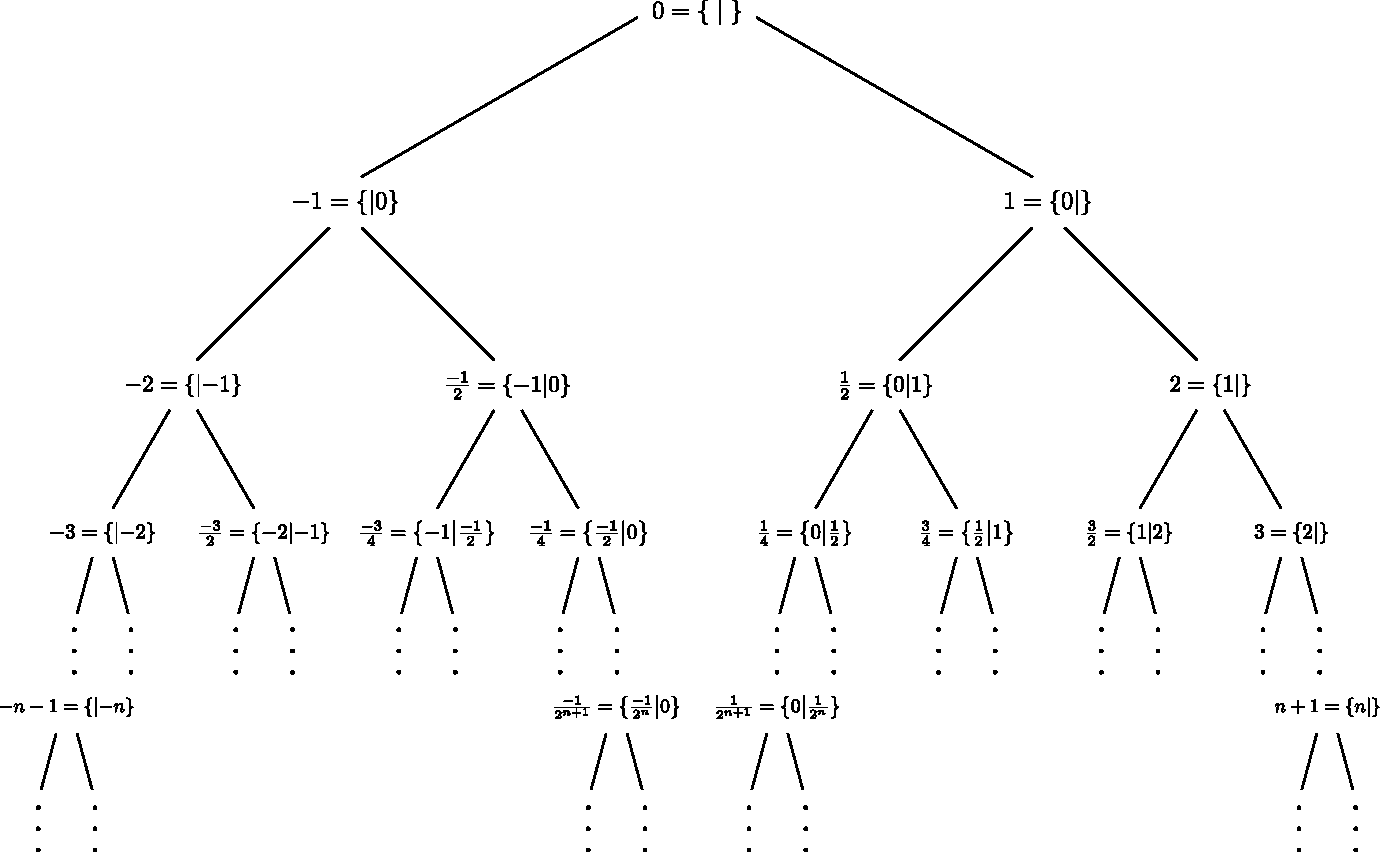
\includegraphics[width=\textwidth]{images/surreal-finite.pdf}
        \caption{Los n\'umeros d\'iadicos como n\'umeros surreales.}
        \label{figure:surreal-finite}
    \end{sidewaysfigure}